\documentclass{article}
\usepackage{graphicx}

\usepackage{longtable}
\usepackage{hyperref}
\begin{document}

\title{Vigenerova šifra}
\author{Martin Klíma}

\maketitle

\section{Výsledky}
\begin{longtable}{|p{0.2\linewidth}|p{0.8\linewidth}|}
    \hline
    Repozitář: & \url{https://github.com/mugac/Vigenere} \\
    \hline
\end{longtable}
\centering
\begin{longtable}{|p{0.1\linewidth}|p{0.9\linewidth}|}
    \hline
    CT: & \texttt{dejlogmnpnnravvncvtkrsegvbcjkrkejuakwejurvenzfvippvt\newline adpskbtepskjnrcycpjrloebskvpejcbzskbttfsbpscpvvosbbp\newline ifdkjmvyijuomblfkabpjvenraeuwolsegvbcjktfsbpscpvvosb\newline ffveeibcvoambzlkekbkvoamjcvoequijjczmekfdvkiezcvtkvt\newline trunfttzbklmtlsygpdcfsmfujuamzjvdejlaifplclzlagbrcbm\newline votejdvnobsakjcbzpibvejskbtjmisfrrmnznskbtejmifzzned\newline bpfmikjcbzmjzskfmvnzrmoqfnpnnrtvfcouoejpukfzzqocjtzd\newline kpdhjurroayoukjhcbvfvskbtlkegseqjdvotifplclzlymscypl\newline ezmrkeujnpnzrloepdrsnpnoihaefmafdmpubpmfsomzprslrnee\newline ucvtkvsegvbcjkpoamscypllnotjvploeoejuoajvcbdrdejleif\newline plclzlytfsbpjvaedfskszejmypsgpdrsskwidltvsagpdcfebpn\newline fnitlytisfdirmnzdhrqocjtzdkpdhzodzlakprlkabpjvidgoaf\newline cymbtvmezodvylzesbfhfsoqwoafieeeotvfcouztztkldizodvy\newline smpbfeyzotvsnvuufecvozlsygbtijkmzsfdeipzmjnluydttruu\newline dtvvuavloepmzdkpqaksiumejwekpvvcaelyupsbvpzoyksitftz\newline keuoaefjsphruszdhjuakvsmftrtnvkvptszniwjnrocejmzqrzk\newline mpwpfsomoaejsajnpnijuakzmrwecnidblpqoujlfcymbtvmzzki\newline tjcyqouqrrieddhleoszvplaqvjvueqqodfrefnzakfvnvsomooj\newline umvaiefjsphruszniroeadhlesznifcymbtvmirsecbtzwnvwymb\newline zvoegseipzuflfwaejbfiakttmjnrqrzdpfqucbczniibnvaadfs\newline koaepskjjvelfvhfeosfnzakrbpfepivmvsedwyjqeczcyaedjvz\newline odvyuvlocpgzdkvttfqyafcvtkfppiptzoebueizmajnpnvptpvm\newline ydaedjmdfnjjmvlocpgzdkpndcvzejkvncvtkfteumolioupbvsa\newline ujmvaigbtebckoeaceqqetoeatitizvniebsmftv} \\ \hline
    Délka klíče: & 3 \\ \hline
    Klíč: & \texttt{abc} \\ \hline
    OT: & \texttt{Česko plným názvem Česká republika je stát ve střední Evropě. Samostatnost nabylo jako nástupnický stát Československa, předtím existovalo jako jedna ze dvou republik československé federace. Navazuje také na více než tisícileté dějiny české státnosti a kultury. Podle své ústavy je Česká republika parlamentní demokratický právní stát s liberálním státním režimem a politickým systémem založeným na svobodné soutěži politických stran a hnutí. Hlavou státu je prezident republiky, vrcholným a jediným zákonodárným orgánem je dvoukomorový parlament České republiky. Na vrcholu moci výkonné stojí vláda České republiky. Česko je země s tržním hospodářstvím, která podle ekonomických, sociálních a politických indikátorů, jako je HDP na obyvatele, index lidského rozvoje, index svobody tisku či index svobody internetu od cenzury, patří k vysoce rozvinutým státům světa. Ekonomicky patří dle Světové banky do skupiny třiceti jedna nejbohatších států světa s nejvyššími finančními příjmy v porovnání s jinými státy. Má velmi malý podíl obyvatel žijících pod prahem chudoby, vykazuje též poměrně nízkou nerovnost mezi nejbohatšími a nejchudšími obyvateli a relativně vyvážené přerozdělování bohatství napříč populací. Míra nezaměstnanosti je dlouhodobě nízká a pod průměrem vyspělých zemí. V indexu ekologické stopy je Česko oproti některým jiným vyspělým zemím menším ekologickým dlužníkem. Česko se dlouhodobě řadí mezi patnáct nejbezpečnějších zemí na světě.} \\\hline
\end{longtable}
\raggedright
\newpage

\section{Řešní}
    \subsection{Délka klíče}
    Pro zjištění délky klíče jsem využil index koincidence (pravděpodobnost, že dvě náhodně vybrané písmena z textu budou stejné). 
    Aby se dala zjistit  délka klíče, je zapotřebí text rozdělit do skupin podle odhadované délky klíče a pro každou skupinu spočítat
    index koincidence a udělat průměr všech skupin. Takto projdeme všechny možné hodnoty (většinou nějaké rozmezí + délky, které můžeme odhadnout 
    napříkald pomocí kasiskiho testu). Výsledky se následně porovnají s indexem koincidence pro jazyk, kterým je psán open text. Délka klíče je 
    pravděpodobně ta hodnota, která se nejvíce shoduje.
    \\
    Index koincidence v čj: 0.058\\
    Index koincidence pro různé délky klíče:
    \begin{tabular}{|p{0.05\linewidth}|p{0.4\linewidth}|}
        \hline
        2 :& 0.045776882608718455 \\ \hline
        3 :& 0.05811856786273908 \\ \hline
        4 :& 0.0463213970495524 \\ \hline
        5 :& 0.045428275949208494 \\ \hline
        6 :& 0.058654984608098516 \\ \hline
        7 :& 0.04508961982327601 \\ \hline
        8 :& 0.04603564788574276 \\ \hline
        9 :& 0.05815838800698883 \\ \hline
        10 :& 0.04552157631571028 \\ \hline
        11 :& 0.04557283982062743 \\ \hline
        12 :& 0.059204264229963825 \\ \hline
        13 :& 0.0458975794642088 \\ \hline
        14 :& 0.045027054180483084 \\ \hline
        15 :& 0.05708591668692233 \\ \hline
        16 :& 0.04735231873389768 \\ \hline
        17 :& 0.04692124454129199 \\ \hline
        18 :& 0.058981166913372886 \\ \hline
        19 :& 0.04549901852533432 \\ \hline
        20 :& 0.04642693460250309 \\
        \hline
    \end{tabular}
    \\
    \subsection{Prolomení klíče}
    Při znalosti délky klíče je možné text dešifrovat několika způsoby. Já jsem využil frekvenční analýzu, která využívá toho, že v 
    každém jazyce se každé písmeno vyskytuje ve své vlastní frekvenci oproti čistě náhodnému textu, kde by frekvence písmen měla být 
    velmi podobná. Text jsem rozdělil do skupin podle délky klíče((1,4,7)(2,5,8)(3,6,9)) a následně na každou skupinu provedl frekvenční
    analýzu, abych získal jednotlivé písmena klíče. Pro zjištění posunu jsem si frekvenci písmen znázornil do grafu a porovnal s grafem
    běžné distribuce písmen v čj. Spoléhat se na frekvenci písmen s vysokým výskytem může být v kratších textech nejisté, proto jsem se 
    zaměřil na nízké výskyty. Páry f-g a w-x, mezi kterými je ještě q mají skoro nulové výskyty, proto jsem je zvolil jako ideální patern
    pro zjištění posunu.\\
    Grafy frekvence písmen:
    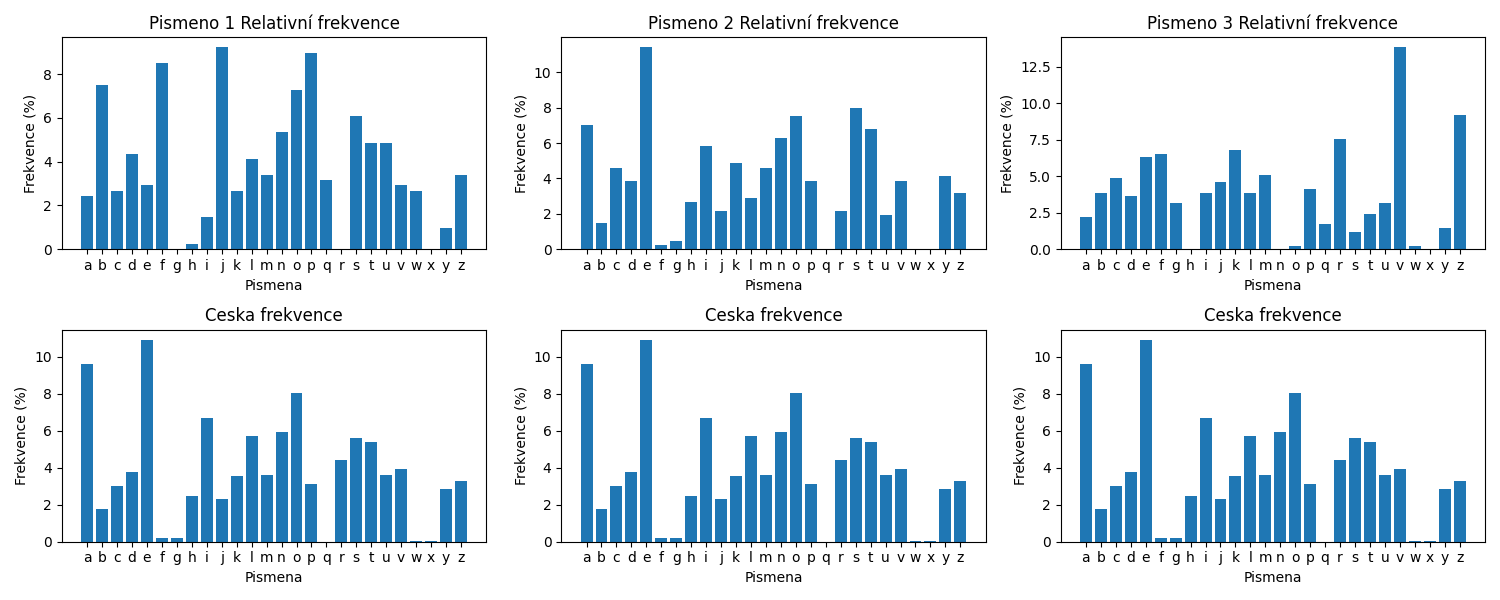
\includegraphics[width = 1.3\linewidth]{FrekvenceGraf.png}\\
    Podle posunů jsem zjistil klíč: bar\\
    \subsection{Dešifrování}
    Když už mám klíč, tak stačí text dešifrovat. Pro dešifrování jsem použil stejný postup jako při šifrování, ale s opačným posunem.
    Pro každé písmeno jsem vzal korespondující písmeno klíče a provedl podle něho posun.\\

\end{document}